\documentclass[a4paper,twocolumn]{esapub2005} % European paper
\pagestyle{empty}

% introduce this option for the ESA publications style
\bibliographystyle{alpha}

\usepackage{graphicx,subfigure} %for figures \usepackage{subfig} %forsubfigures
\usepackage[fleqn]{amsmath}    % need for subequations
\usepackage{multirow} % for complex tables \usepackage{multicol} % for columnsspliting
\usepackage{color} %for highlight text \usepackage{booktabs}
\usepackage{url}
\usepackage{units}
\usepackage{floatrow}
\usepackage{float}

\graphicspath{{img/}}
\restylefloat{table}

\title{First Experimental Investigations on Wheel-Walking for Improving
Triple-Bogie Rover Locomotion Performances}

\author[1]{Martin Azkarate}
\author[1]{Martin Zwick}
\author[2]{Javier Hidalgo-Carrio}
\author[1]{Robin Nelen}
\author[3]{Tim Wiese}
\author[1]{Pantelis Poulakis}
\author[1]{Luc Joudrier}
\author[1]{Gianfranco Visentin}
\affil[1]{European Space Agency, ESA, Noordwijk, The Netherlands}
\affil[2]{Robotics Innovation Center, DFKI, Bremen, Germany}
\affil[3]{Technische Universit\"at M\"unchen, TUM, Munich, Germany}


\newcommand{\btx}{\textsc{Bib}\TeX} \newcommand{\filename}{esapub}

\begin{document}

\keywords{\LaTeX; ESA; macros}

\maketitle

\section*{Abstract}

\textbf{Deployment actuators of a triple-bogie rover locomotion platform can be used to perform Wheel-Walking (WW) manoeuvres. How WW could affect the traversing capabilities of rovers is a recurrent debate in the planetary robotics community. The Automation and Robotics Section of ESTEC has initiated a long term project to evaluate the performance of WW manoeuvres in different scenarios. This paper presents the first experimental results on this project, obtained during the test campaign run on November 2014 at the Planetary Robotics Lab (PRL) of ESTEC, and shows the performance analysis made when comparing WW with standard rolling.}

\section{Introduction}

Planetary rover missions to Mars such as NASA's MER or MSL have shown a clear decrease of the traversing capabilities while rolling across some particular surface areas of Mars. Loose soil and fine dust terrain is the scenario where rovers may experience the most significant loss of their tractive performance. The extreme of these cases was encountered in the Spirit rover which got permanently stuck on May 2009 while traversing the loose sandy area of Troy ~\cite{SpiritTrap}.

%================================================================
%Previous studies at JPL ~\cite{ROB:ROB21481} introduce the concept of the Effective Ground Pressure (EGP) as a first order of approximation for an inversely proportional indicator of the traversing capabilities of a rover. In relation to this, ExoMars' estimated EGP (considering an effectively larger wheel due to its flexible properties) is about 2.5 times the one of MER and MSL.
%================================================================

Following the Lunokhod mission, Russian engineers developed numerous planetary exploration rover concepts where they demostrated major increase in gradeability and obstacle negotiation performances by implementing a "peristaltic" locomotion mode in some or a "wheel-walking" mode in others ~\cite{Ehrenfreund1998}. The triple-bogie rover concept was conceived in the early phase of the ExoMars mission ~\cite{Patel2010} and has become the baseline for the rover's locomotion. Moreover this type of suspension has become widely accepted in the European space robotics community due to good locomotion performances and design simplicity. The location of the deployment actuators of the triple-bogie concept offers the WW mode for free and this is another great benefit of this suspension concept.

Based on the above and given that the triple-bogie concept will probably have a role in future European exploration missions, the Automation \& Robotics Section has initiated a long term internal project to characterize the performances of this suspension concept. A significant part of this project focuses on the WW mode with the aim to fully understand and exploit its potential.

The target platform for the initial test results of this investigation on the WW mode is a triple-bogie laboratory prototype, namely ExoTeR. 

%================================================================
%Deployment actuators of a triple-bogie rover locomotion platform could in
%principle be used to perform wheel-walking manoeuvres.  How wheel walking could
%affect the traversing capabilities of rovers when driving on the aforementioned
%disadvantageous terrain types is a recurrent debate in the planetary robotics
%community. The Russians Lunokhod and Marsokhod rovers already used in the past
%a locomotion concept named peristaltic motion very similar to the wheel walking
%concept explained in this paper  with which they claimed to gain "amazing
%slope climbing and obstacle overcoming capabilities".
%
%This led the Automation \& Robotics Lab of ESTEC to initiate an internal
%project aiming at the development of wheel-walking control algorithms and the
%assessment of the subsequent locomotion performances. The target platform of
%this investigation is a triple-bogie laboratory prototype, namely ExoTeR.
%================================================================

This paper briefly presents the ExoTeR rover in section 2, the WW
concept in triple-bogie locomotion configurations in section 3 and focuses in
section 4 on the first experimental results obtained for three different
operational scenarios, comparing key performance metrics between the wheel
walking and rolling locomotion modes. The three operational scenarios
considered are: 1) entrapment in loose sand, 2) up-slope traverse and 3) rover
egress. Section 5 gives the conclusions drawn from these experiments and in
section 6 the future work and test plan is explained.

\section{The ExoMars Testing Rover}

The rover platform used for the experiments described hereafter is an
ExoMars-like scaled down version laboratory prototype. The ExoMars Testing
Rover (ExoTeR)~\cite{Azkarate2015} mimics the locomotion configuration of
ExoMars (according to its design in 2007), a.k.a. triple-bogie passive
suspension, with a parallelogram structure on top of each bogie. The locomotion
subsystem comprises 6 wheels and 16 actuated joints, more precisely, 6 driving,
4 steering and 6 deployment (or walking) motors.  Motion control electronics
are a network of servo-drives, namely Elmo Whistles, connected in a CAN Bus
together with the On-Board Computer (OBC). A driver module in the OBC acts as a CAN
Master implementing the CANOpen protocol and sends joint commands timely
synchronised to perform a certain locomotion manoeuvre. Each servo-drive takes
care of the close-loop control of one active joint to reach the commanded
(position and/or velocity) set point.  Figure \ref{fig:ExoterRover2013} illustrates the locomotion
system of ExoTeR. Inside the uncovered body the motion control electronics can
also be seen.

\begin{figure}[h!]
    \centering
    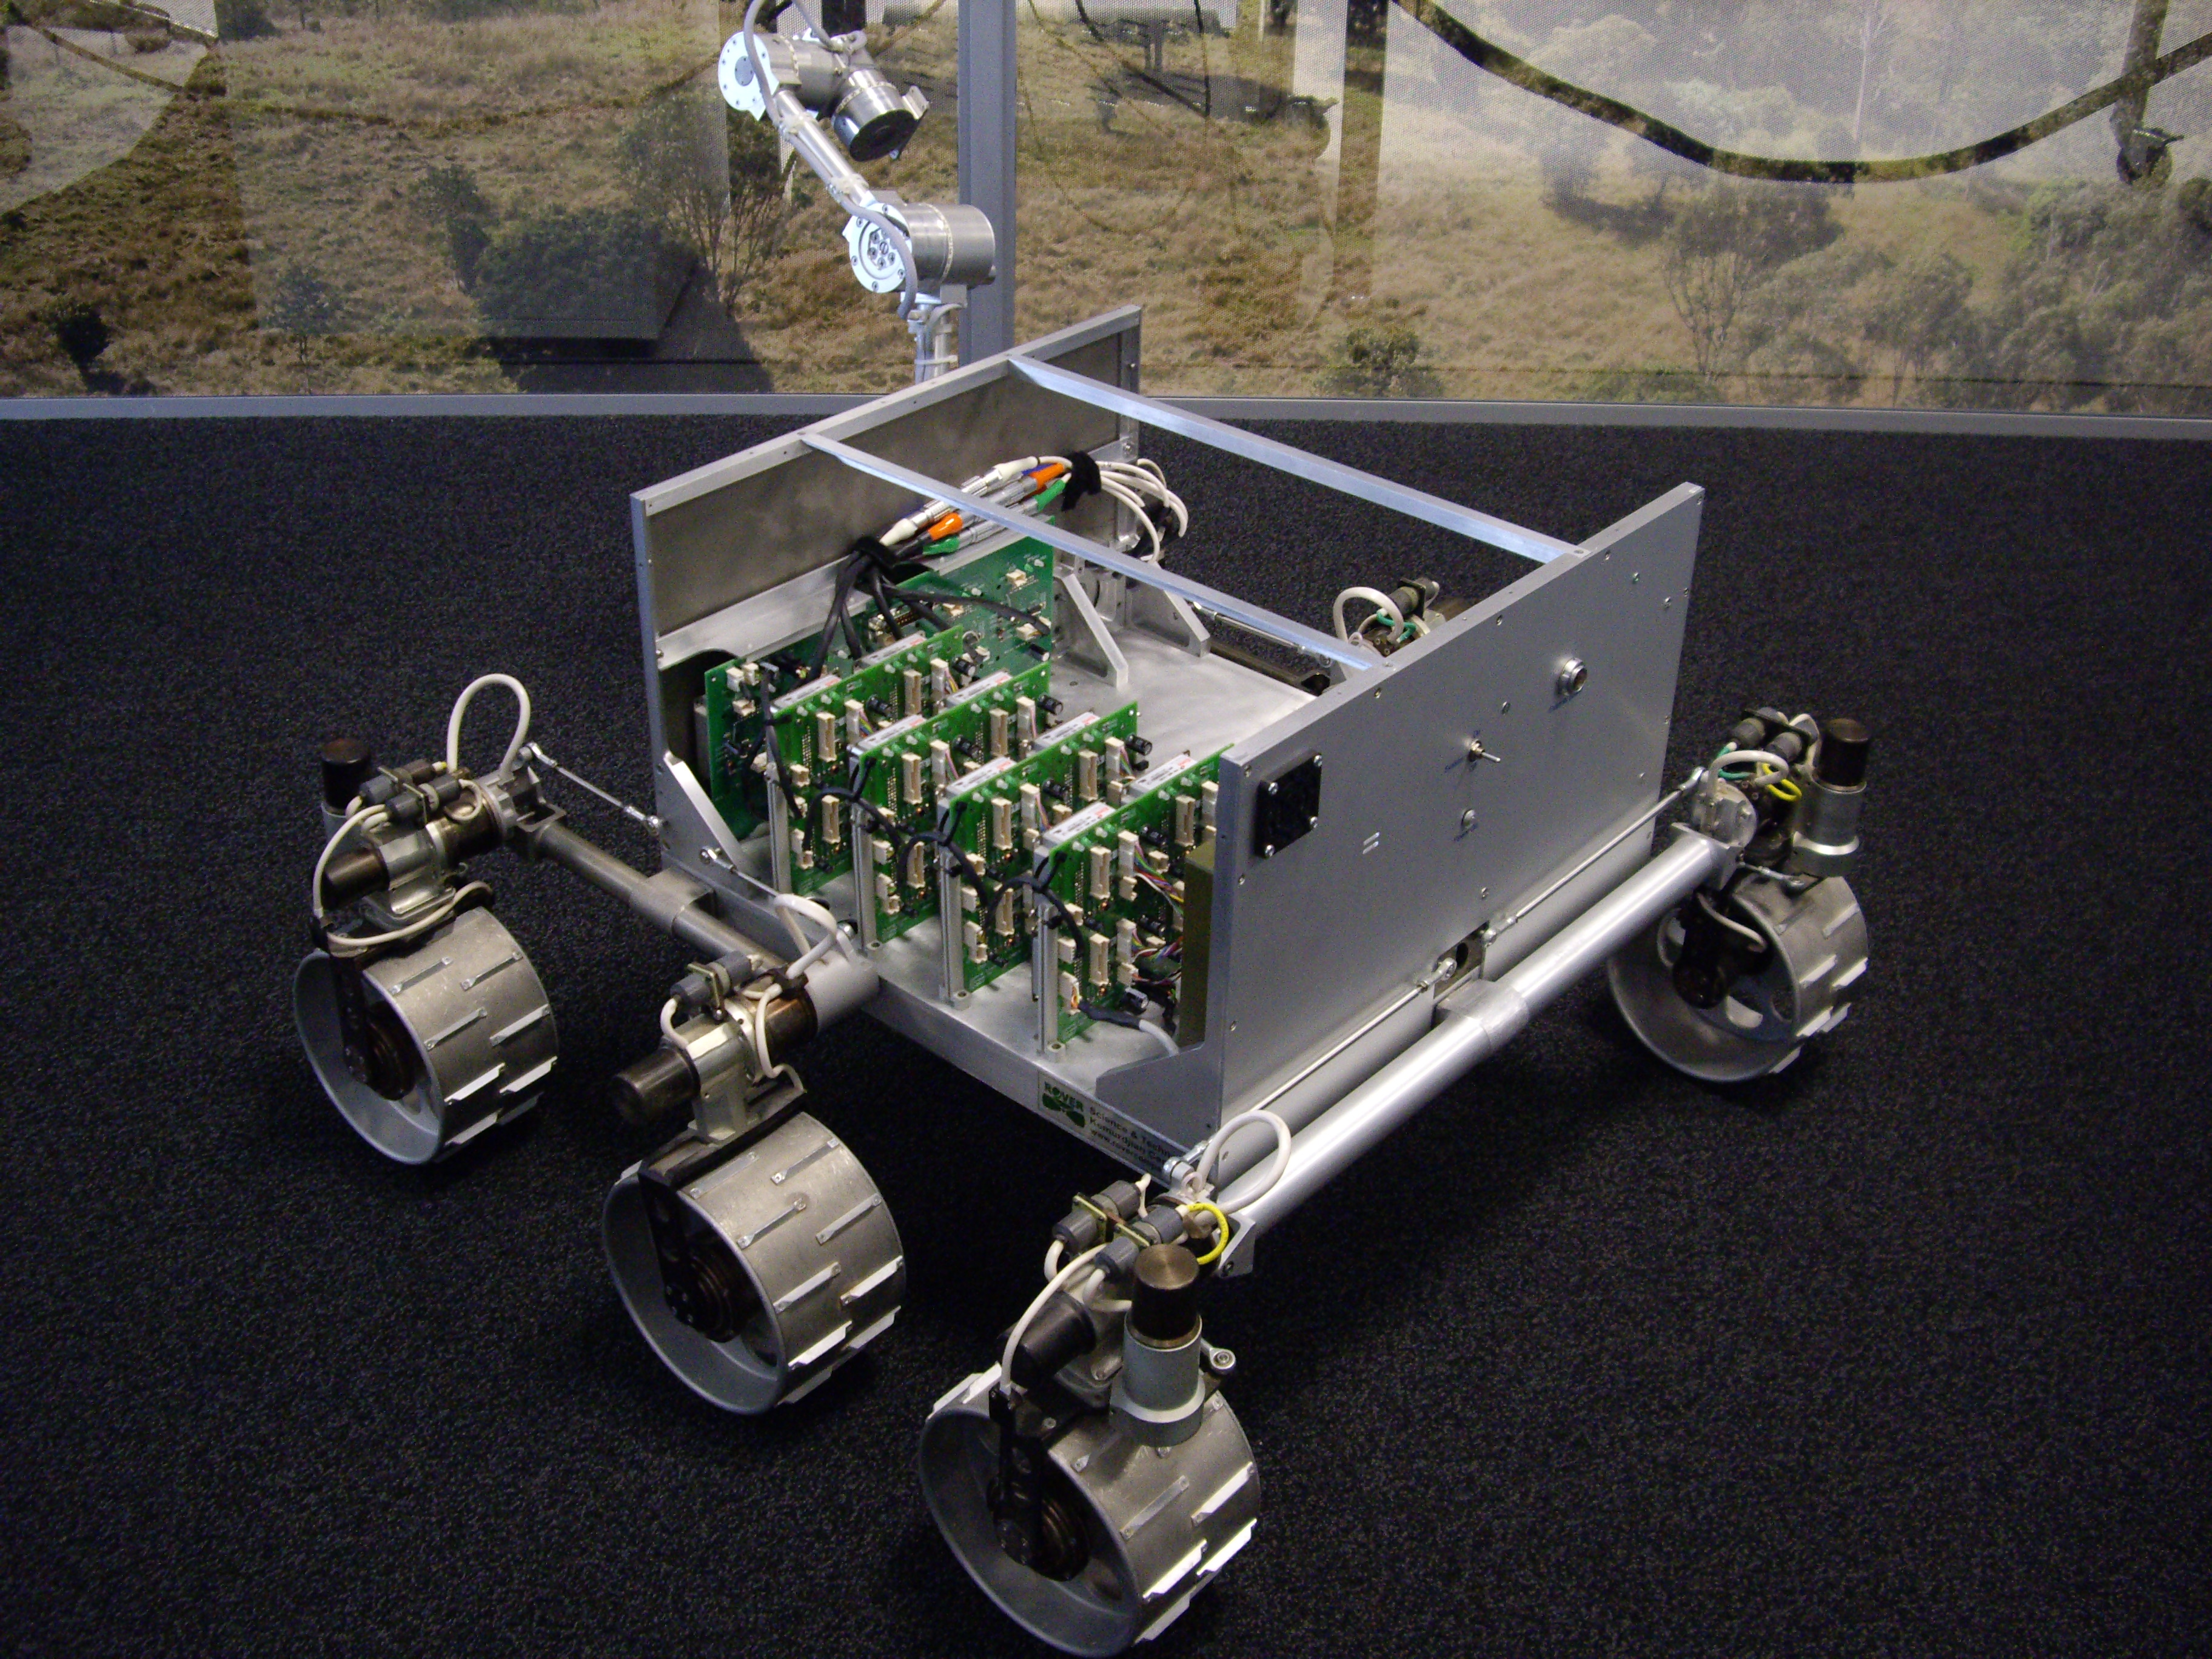
\includegraphics[width=0.9\textwidth]{ExoterRover2013.jpg}
    \caption{ExoTeR Rover, 2013}
    \label{fig:ExoterRover2013}
\end{figure}

The general dimensions of the rover are summarised in table \ref{tab:ExoterDimensionsTable} below. The ground pressure calculation is based on the Effective Ground Pressure convention defined by JPL in ~\cite{ROB:ROB21481}.

\begin{table}[h]
	\begin{tabular}{ll}
	Locomotion platform type       & $6~\times~4~\times~6$             \\
	Size ($L~\times~W~\times~H$)   & $70~\times~70~\times~40$ ~\unit{cm$^3$} \\
	Wheel diameter                 & 14 ~\unit{cm}    \\
	Wheel width                    & 9 ~\unit{cm}     \\
	Total mass                     & 24.08 ~\unit{kg} \\
	Ground pressure                & 6.25 ~\unit{kPa}        
	\end{tabular}
	\caption{Rover characteristics and dimensions}
	\label{tab:ExoterDimensionsTable}
\end{table}

The rover system currently includes a 5 DoF anthropomorphic arm and a mast structure and PTU mechanism with mechanical interfaces to attach a stereo camera and a ToF camera as well. Other sensors include an Inertial Measurement Unit, and incremental encoders and absolute position sensors for the active and passive joints of the locomotion kinematic chain. For the acquisition of the ground truth data inside the lab the Vicon Tracking System is used. For outdoor testing the OBC has integrated a D-GPS receiver with \textit{rtk} corrections. The control architecture of the rover, which comprises the functional layer for now, is implemented using the Rock robotic software framework ~\cite{}. The system is used to perform R\&D activities in the fields of: system integration, locomotion performance, control architecture design and implementation, and sensor data fusion among others. 

\section{Wheel Walking Implementation}

Global body commands of motion are commonly performed using a motion model.
Kinematics motion models have real-time capabilities and are inexpensive in
comparison with sophisticated wheel-dynamic simulation techniques.  The
WW evaluation presented in this paper uses a method which is able to
\textit{optimally}\footnotemark[1] combine the motion induced at each contact
point. The primary contribution of the model is fusing, in a unified framework,
desired body velocities to joint motion commands as a whole.  The
implementation of a complete motion model behaves more consistent and stable
than previous WW techniques. The model makes use of the
transformation approach~\cite{Tarokh2005} to accurately model 6-DoF kinematics.
It derives from the work in~\cite{Hidalgo-Carrio2014} to invert the Jacobian
formula from the odometry kinematics.

The model requires a minimum of two coordinate frames per kinematic chain: a
robot body frame ($B$) attached to the desired rover center and a contact frame
($C_{il}$) defined as a single point of contact between the robot and the
ground. Those coordinate frames are related to each other by means of the
Jacobian matrix in the velocity domain. The matrix maps Cartesian to joint
velocities and relates the rover pose rates to joints and sensed rate
quantities as:

\begin{equation}
    \left[\dot{x}_{B} ~ \dot{y}_{B} ~ \dot{z}_{B} ~ \dot{\phi}_{B}
    ~ \dot{\theta}_{B} ~ \dot{\psi}_{B} ~ \right]^T = J_{il}
    \left[\boldsymbol{\dot{q}} ~ \boldsymbol{\dot{\varepsilon}}_{il} \right]^T
    \label{eq:wheeljacobian}
\end{equation}

where $\boldsymbol{\dot{q}}$ are the desire joint rates to command to the
actuators.  Different WW gaits (i.e. motion patterns ~\cite{LucWalkingGaits}) are set by
dynamically setting constraints in the Jacobian. Each Jacobian defines the
contribution of each kinematic chain to the body motion allowing the analysis
of each chain and contact point to the resulting final velocity in the robot
body.  Considering a single contact angle $\dot{\varepsilon}_{il}$ the $J_{il}$
matrix size is $6 \times (n + 6)$ where $n$ corresponds to the DoF of the
mechanism.  The composite rover equations are obtained combining the Jacobian
matrices for all kinematic chains into a sparse matrix equation of appropriate
dimensions. The desired solution is obtained by numerically solving a system of
equations using Weighted Least-Squares.


\footnotetext[1]{Optimally here refers to the best estimated value from a
weighted least-squares perspective.}

\section{Experimental results}

Three different scenarios are considered to evaluate the traversability
performance of the WW locomotion mechanisms, each of them referring
to situations where the rover could potentially benefit from the WW
actuation.

\subsection{Immobilization situation} 

\subsubsection{Objective} This test aims at simulating a trapped situation
from which the rover should free itself. It is the first WW
performance test executed with ExoTeR. The baseline of the test is to verify
the operative readiness of the implemented WW algorithms in a load
wise representative environment.
No numerical metric will be measured in these tests. Only for qualitative purposes the time that the rover takes to get unstuck will be observed, if it gets unstuck at all.

\subsubsection{Setup} The test facility is improvised in an outdoor volleyball
court on a sunny day (see picture \ref{fig:volley}). The sandy part the rover
is driving on has no overall slope. The soil is a normal beach volleyball
silica sand with a mixed grain size of 0.063 - 2.0~\unit{mm}. Due to previous rainfall
some days before, the soil is slightly moist and develops cohesive properties
as seen in picture \ref{fig:volleyexoterdigg}. 

\begin{figure}[h!]
    \centering
    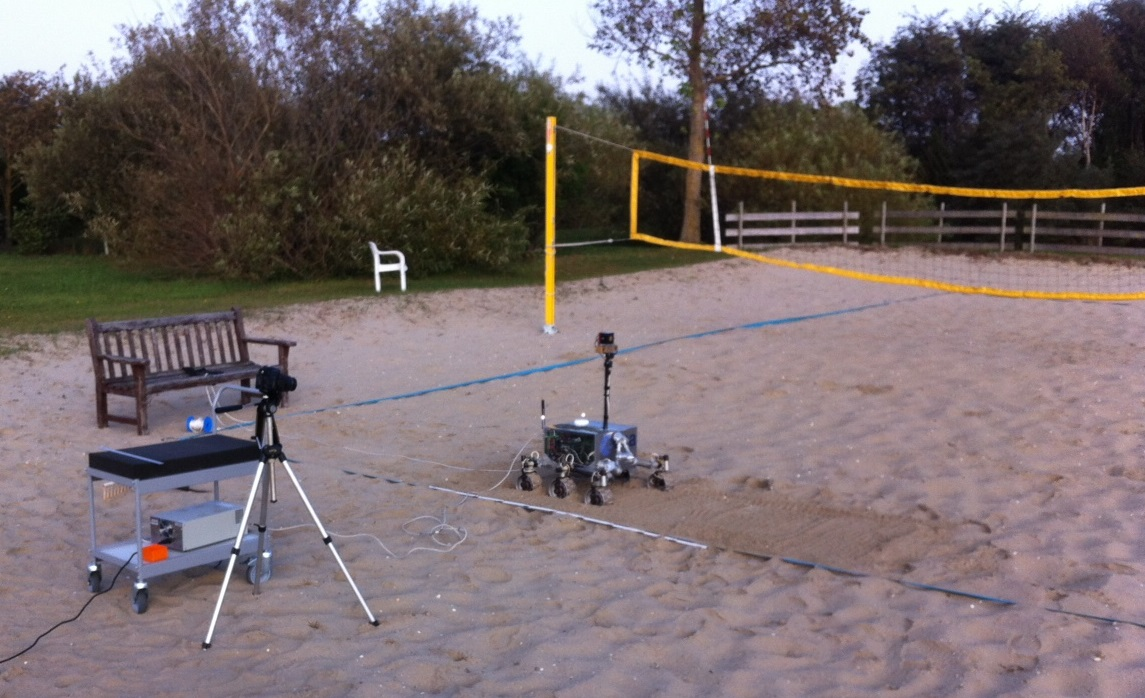
\includegraphics[width=0.9\textwidth]{volley.jpg}
    \caption{Setup on outdoor beach volleyball court}
    \label{fig:volley}
\end{figure}

%The rover was tested on a quartz sand with quartz gravel similar to the
%outdoor beach volleyball sand. The objective of the test was to verify the
%operative readiness of the implemented WheelWalking algorithms in a load wise
%representative environment. Picture \ref{fig:volley} shows the used setup. It
%consists of the ESTEC beach volleyball court, a bench, a camera, a power
%supply, a generator (not in the picture) and a ground control station (not in
%the picture).

%Soil BeachVolleyball: Silica sand [dry and moist], grainsize:0.063 - 2 mm ,
%wet/moist => cohesive soil

The sand gets equally prepared with a raking procedure into approximately 10~\unit{cm} depth before each run.  The rover is commanded \textbf{wireless} and runs on battery. No ground truth system is used in this experiment. The used procedure is divided in two characteristic parts. The first part is to get the rover stuck in a repeatable way. Therefore the rear bogie is tied to the bench with a detachable rope. With the rope on tension, the rover starts driving away from the bench. Once the drawbar pull and the tension have the same value, the rover does not produce any forward motion anymore and keeps digging itself into the ground as shown in Figure \ref{fig:volleyexoterdigg}. This stops once the rear wheels are sunk by half their diameter into the soil. After that, the rope gets untied and part two starts. The system restarts in normal driving (ND) or WW mode and the data starts being recorded. 

\begin{figure}[h!]
    \centering
    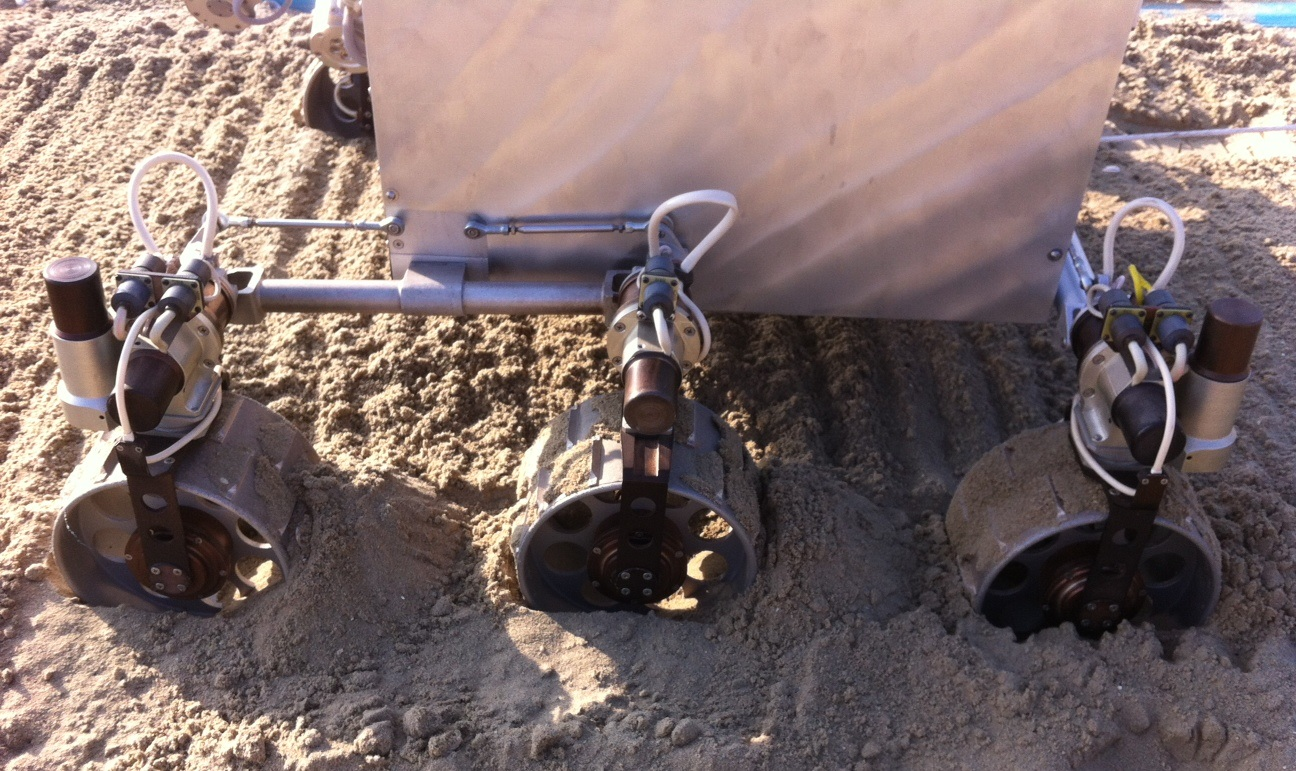
\includegraphics[width=0.9\textwidth]{volleyexoterdigg.jpg}
    \caption{ExoTeR bogged down by half a wheel diameter}
    \label{fig:volleyexoterdigg}
\end{figure}

\subsubsection{Results} As already mentioned both locomotion modes, i.e ND versus WW, are compared (used WW gait is syde-by-syde or left-right ~\cite{LucWalkingGaits}). Both are commanded at a 2 ~\unit{cm/s}
body velocity.

\begin{figure}[h!]
    \centering	
    \subfigure{
        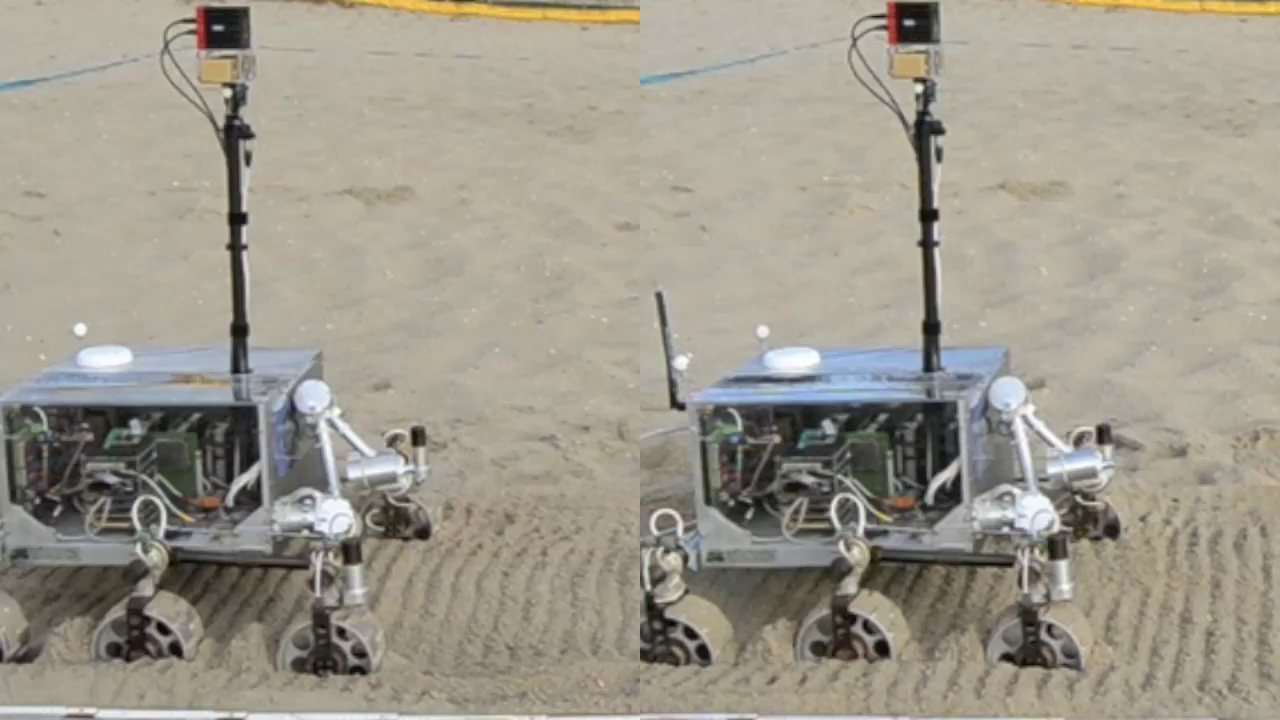
\includegraphics[width=0.45\textwidth]{volleystuck00.png}
        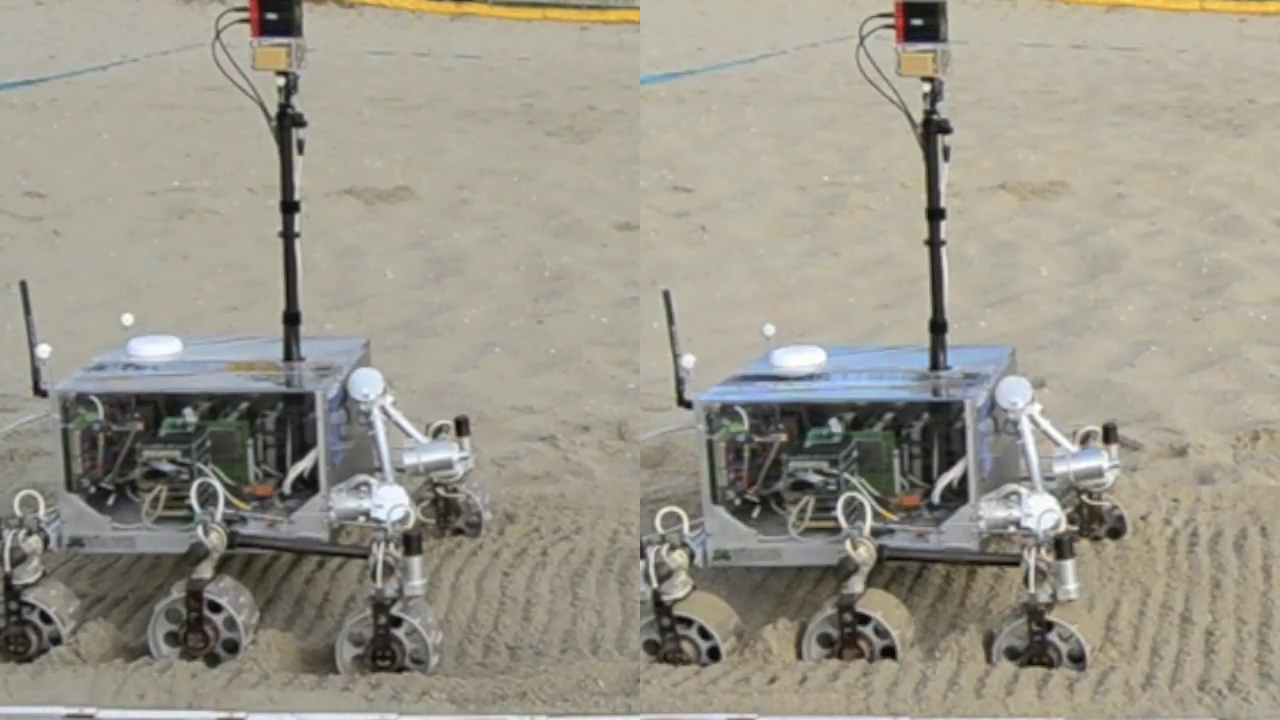
\includegraphics[width=0.45\textwidth]{volleystuck15.png}
    }	
    \subfigure{
        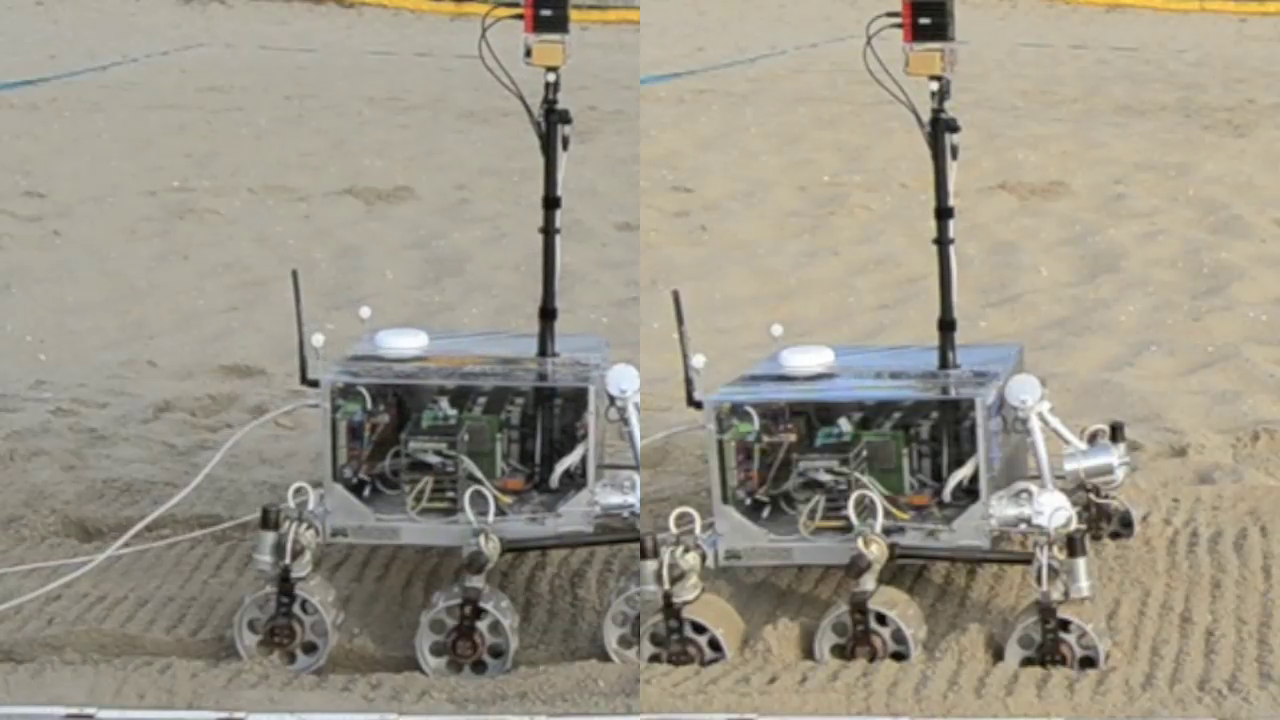
\includegraphics[width=0.45\textwidth]{volleystuck30.png}
        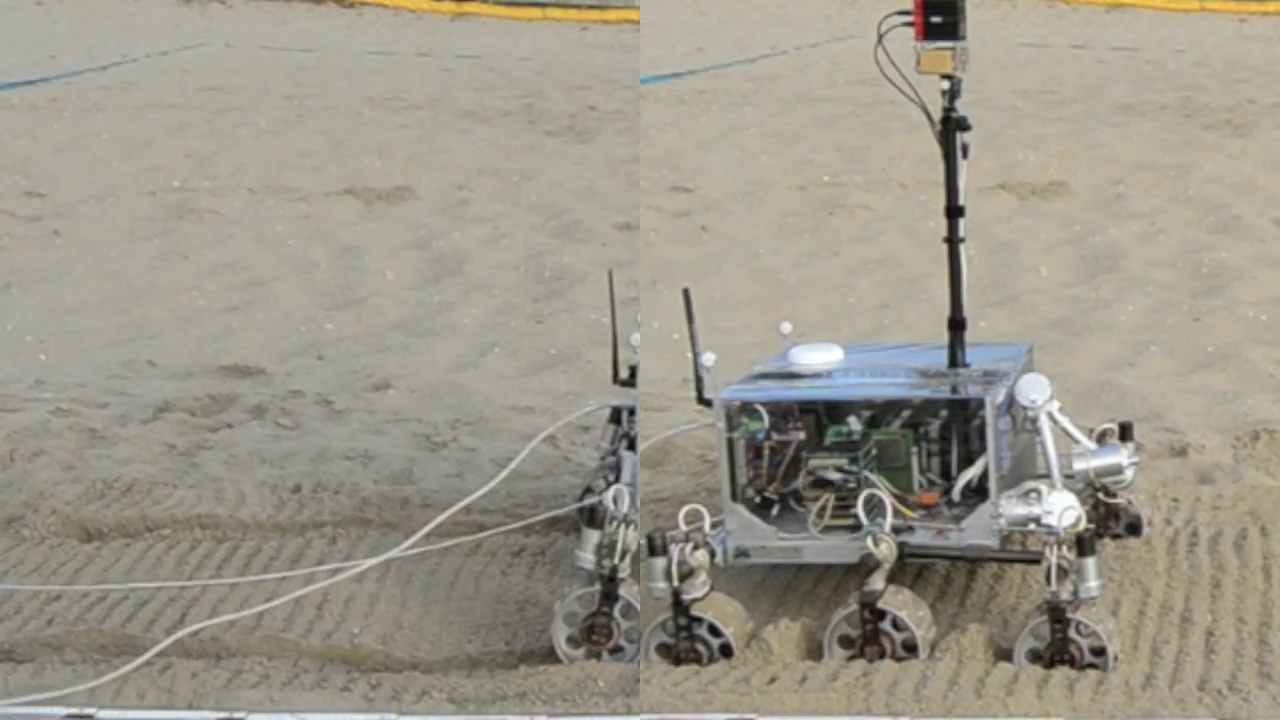
\includegraphics[width=0.45\textwidth]{volleystuck45.png} }
        \caption{top-left:t=0s,  top-right:t=15s, bottom-left:t=30s,
        bottom-right:t=45s; each picture has WW on the left half and
        ND on its right half }
    \label{fig:volleysequence}
\end{figure}

The photo array in figure \ref{fig:volleysequence} shows the progress of the
two modes, ND and WW while trying to set the rover free.
The result is a tremendous benefit of WW. After 45 seconds, normal
driving reaches 3~\unit{cm} and thereby averages a 97\% slip ratio. The WW
run is completely freed after 20 seconds. Assuming that under normal
circumstances, the rover gets trapped while ND, it would be even
more unlikely that it would be able to free itself without WW.

%The metric for this test had a binary format. On the one hand, the rover
%failed to get out of the stuck ( $ > 99 \% $  slip ratio) situation using
%standard driving actuation. On the other hand, using wheel walking locomotion
%in approx. 20 seconds the rover was able to overcome the situation and achieve
%to perform at commanded rover body velocity ( $ < 10 \% $ slip ratio).

%================================================================
%================================================================
\subsection{Gradeability Tests}

\subsubsection{Objective}
Areas with high inclination are particularly interesting to test rover
capabilities for planetary exploration. The objective of the experiments is to test the WW capability on slopes with the aim of evaluating if the maximum gradeability of the system can be increased by means of WW. As metric for these tests the slip-ratio will be accurately measured using the motion tracking system (Vicon) of the Planetary Robotics Lab (PRL). The slip-ratio will be computed as shown in formula \ref{eq:slip}. This unit will be used in the results section for comparison.

\begin{equation} slip = 1- \frac{real\, position\, tracked\, by\,
cameras}{position\, estimated\, by\, wheel\, odometry} \label{eq:slip}
\end{equation}

The motors consumption, although measured, it is not used as a metric for these tests and therefore not shown in the results section. Therefore, this tests do not aim to measure the efficiency of the locomotion modes in terms of power consumption but rather to check if WW mode could be used in some extreme cases enabling the traverse where the ND would not be able to perform\footnotemark[2].

\footnotetext[2]{A traverse stint with slip-ratio higher than 90\% is considered not-performing.}

\subsubsection{Setup}
%placing, soil preparation, gaits, number of repeatings, abort cirieria, 

The rover has to drive from the bottom to the top
of the slope in two modes and successfully repeat this three times per mode.
First the rover performs the traverse three times in ND mode
followed by three tests in WW mode. The tests are done on
0$^{\circ}$, 10$^{\circ}$, 15$^{\circ}$ \& 20$^{\circ}$ slope angles. 

The different slope angles are realized with a soil filled one axis automotive trailer (see photo
\ref{fig:trailer}). Its pivot is the single axis which allows an inclination
from approximately -10$^{\circ}$ up to +25$^{\circ}$. Due to the limited
bearing capacity of the trailer, only a 2~\unit{m} $\times$ 1.1~\unit{m}
$\times$ 0.25~\unit{m} (length $\times$ width $\times$ depth) is filled with
soil. Cardboard boxes fill the leftover volume. In this setup, the filling
depth is more than twice the wheel diameter and the distance to any walls
during a test run is high enough to assume  the boundary effects to be
negligible.  

\paragraph{Soil characteristics} The used soil is 80\% ES3-OMR from Sibelco Ltd mixed with 20\%
gravel provided my KIBAG Zentrallabor. The gravel has a grain size distribution
of 16\% 0-4~\unit{mm}, 18\% 4-8~\unit{mm}, 15\% 8-11~\unit{mm}, 21\%
11-16~\unit{mm} and 30\% 16-22~\unit{mm}.  

The ES3 itself simulates a coarse sandy to gravelly material occurring in scree, polymodal surficial lags and local coarser aeolian accumulations. The coarse scree and aeolian accumulations can occur in terrain with rocky escarpments \cite{michaud2014}.


%Soil ES3-OMR with gravel: Full description of this soil: OMR DRY (from Sibelco
%Ltd, United Kingdom) 80% by mass, with uniformly admixed Hart-splitt gravel,
%16% 0-4 mm, 18% 4-8 mm, 15 % 8-11 mm, 21% 11-16 mm, 30 % 16-22 mm (from KIBAG
%Zentrallabor, Switzerland).

 %ES3 is a coarse sandy to gravelly material occurring in scree, polymodal
%surficial lags and local coarser aeolian accumulations. The coarse scree and
%aeolian accumulations can occur in terrain with rocky escarpments [MI14].

\begin{figure}[h!]
    \centering
    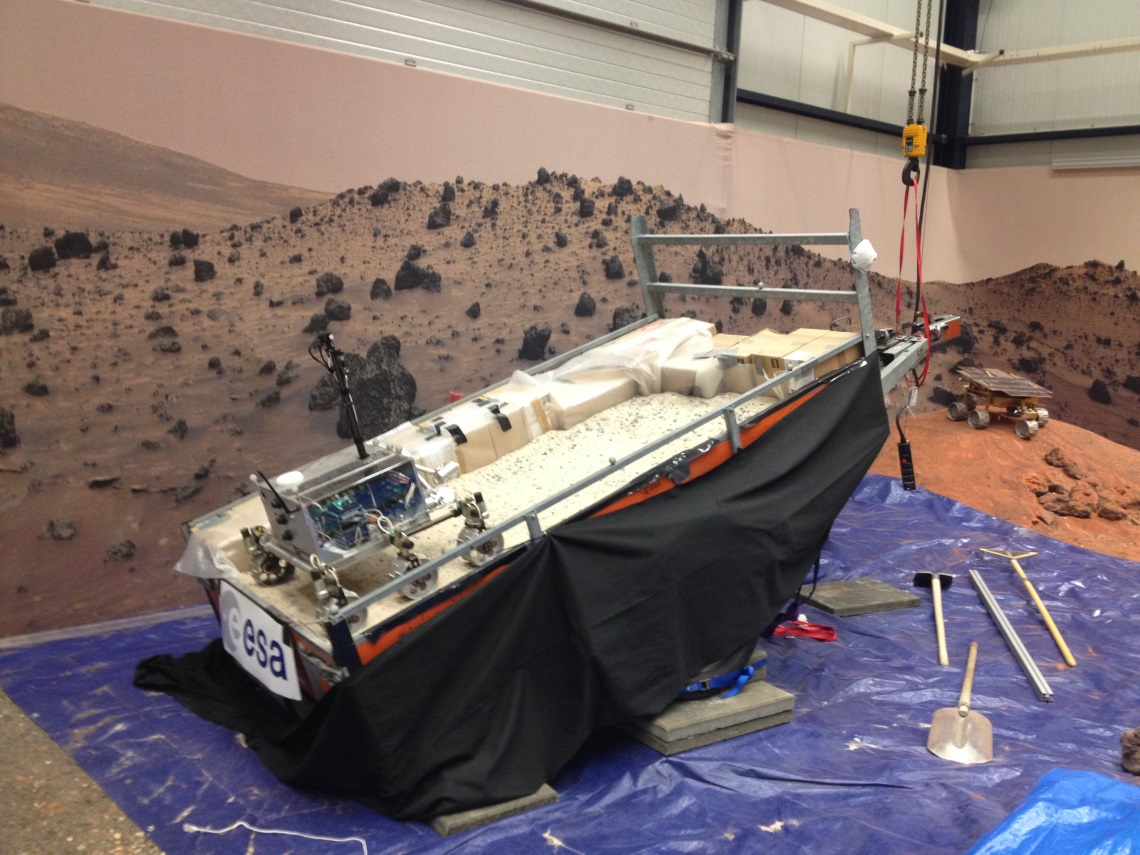
\includegraphics[width=0.9\textwidth]{trailersetup.jpg}
    \caption{Trailer in ESTEC's PRL}
    \label{fig:trailer}
\end{figure}
%_____________________________________________________________

Prior to the hereafter analysed tests, preliminary runs were executed on a
17.5$^{\circ}$ slope to roughly define the most performing WW gait (see figure \ref{fig:Exoslope}).  The side-by-side gait performed best in terms of slip and heading stability and was therefore chosen. 

\begin{figure}[h!]
    \centering
    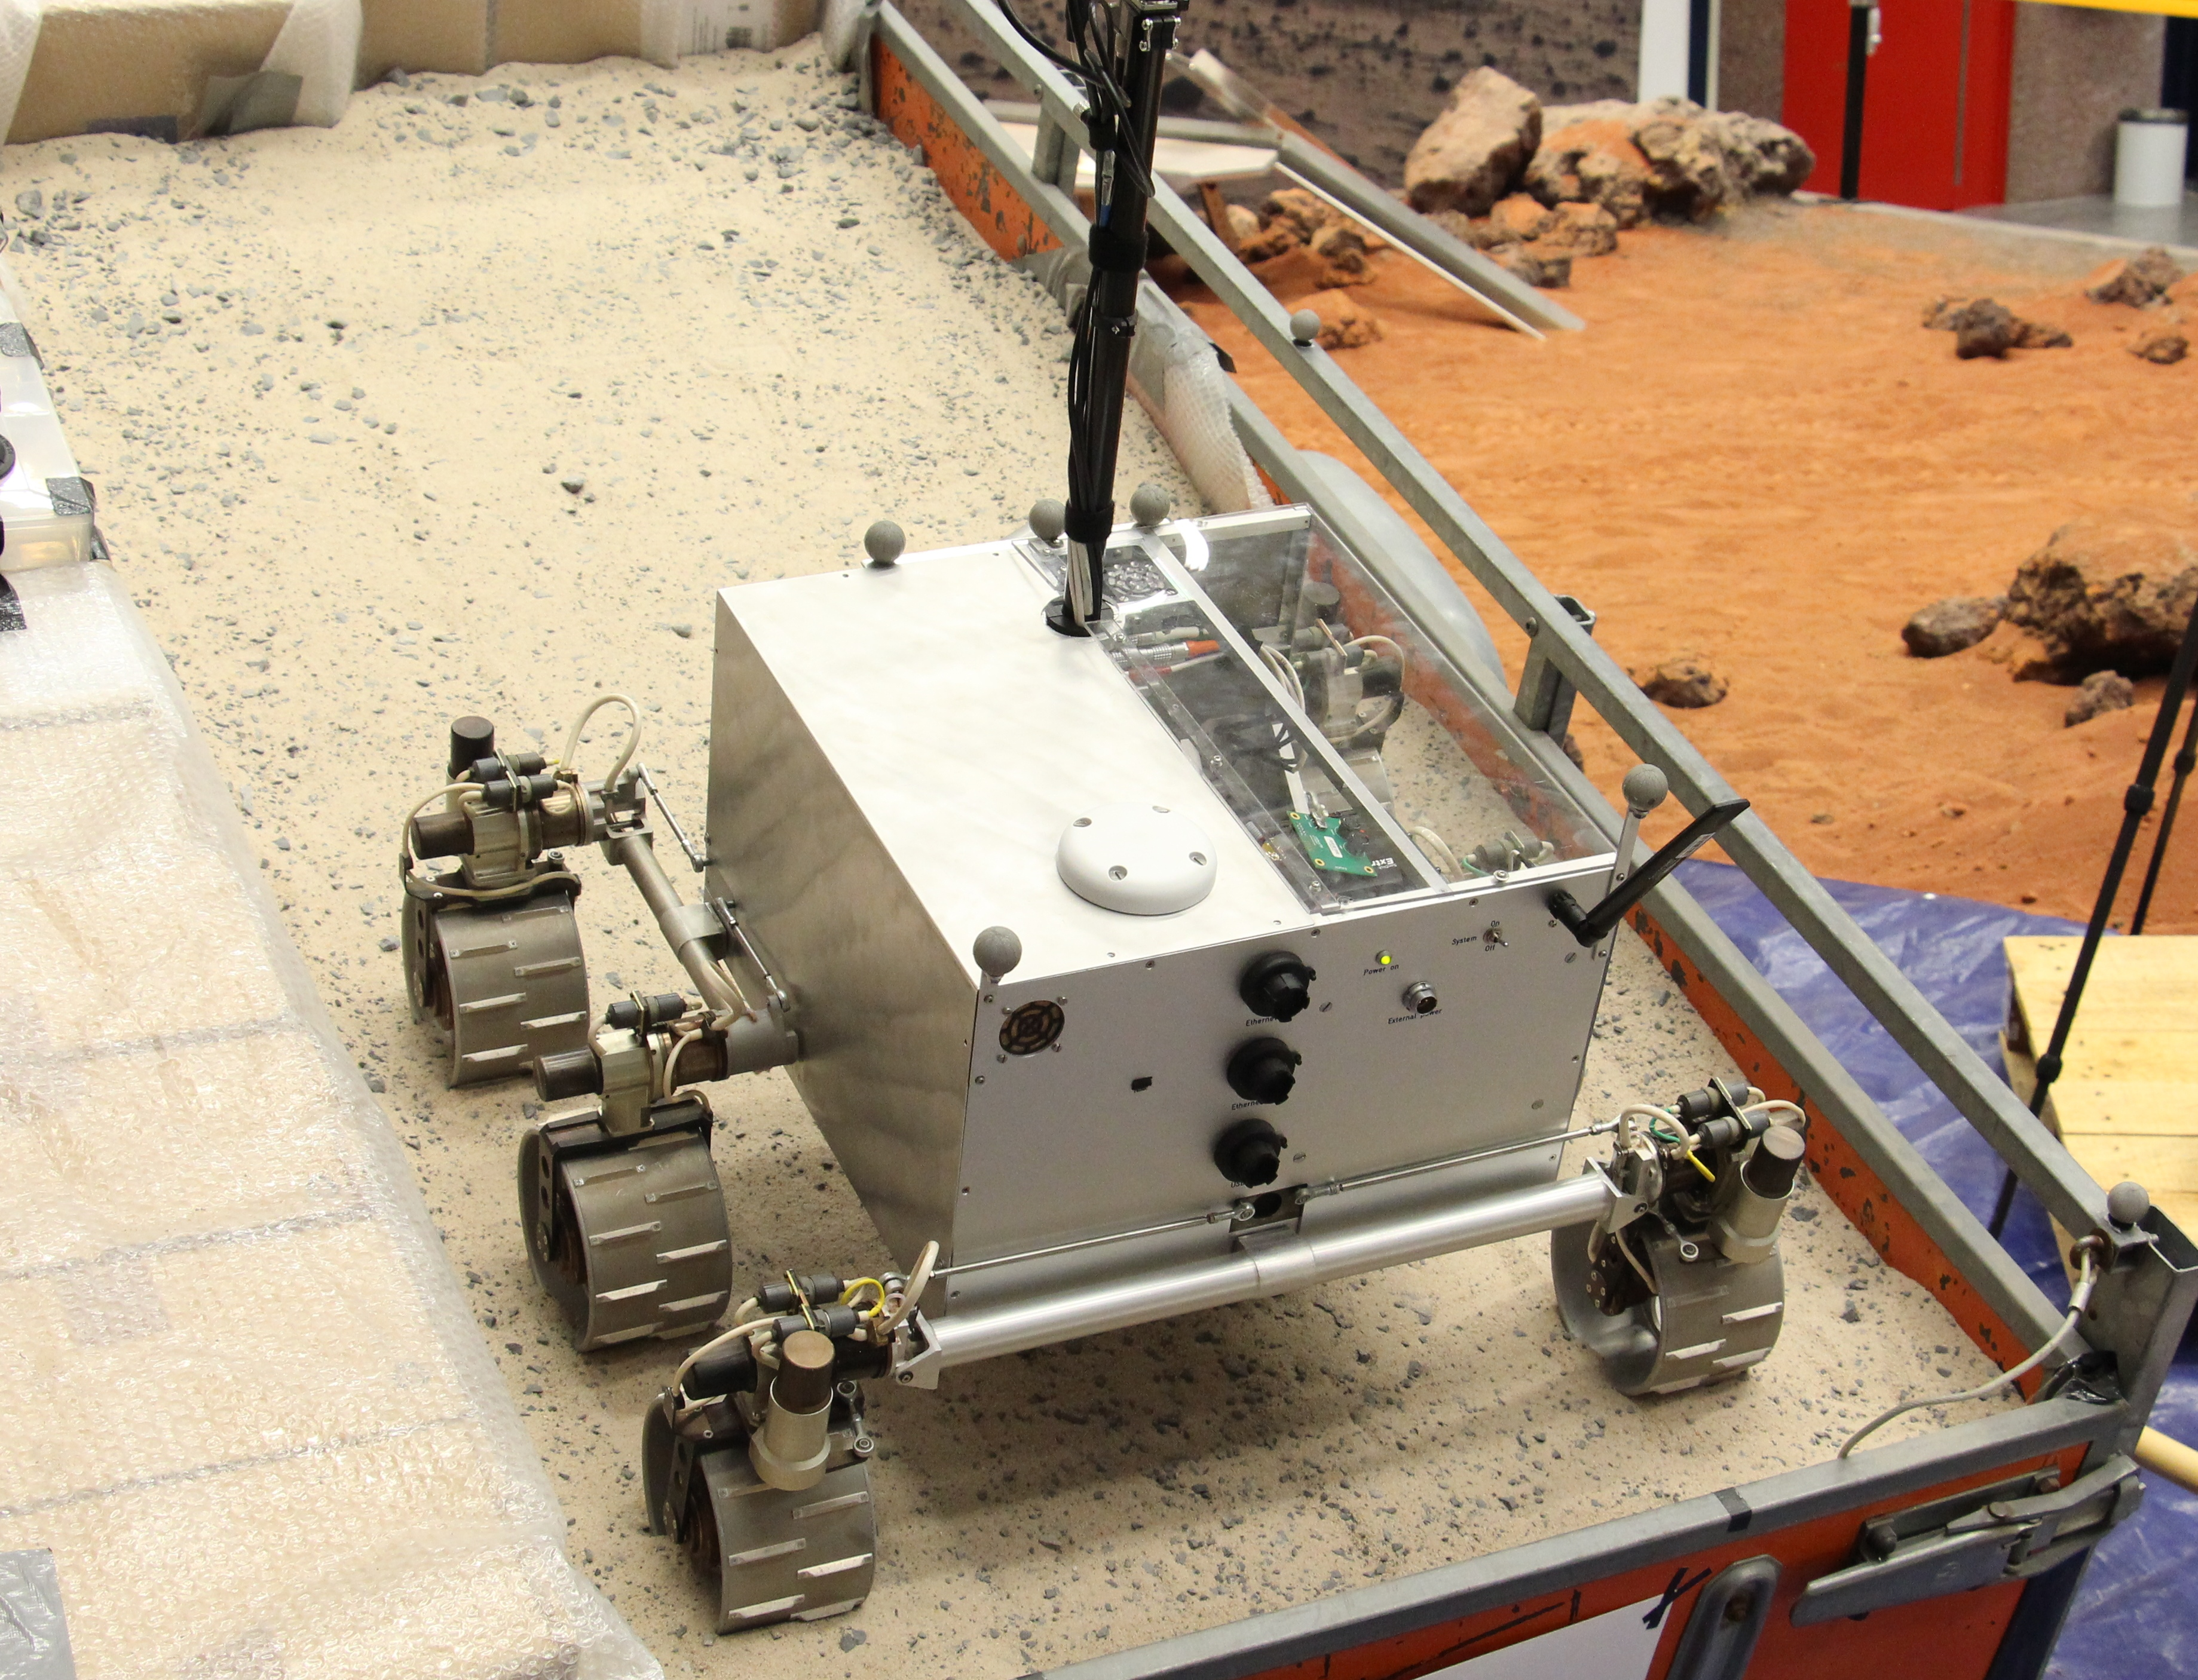
\includegraphics[width=0.9\textwidth]{Exoslope.jpg}
    \caption{ExoTeR rover on 17.5$^{\circ}$ slope in the trailer}
    \label{fig:Exoslope}
\end{figure}

\subsubsection{Results} 
%Other gaits were also used on the dry run tests and after the plan for slope
%tests had been completed. All other tested gaits (AXLE_BY_AXLE and EVEN_ODD or
%TRIPOD) showed to have worse performance in the preliminary tests, i.e. higher
%slip ratios. 
The following subsections show for each of the tested slope angle degrees the resulting slip ratios obtained for ND and WW. All off them show three valid WW tests and three ND tests. These sets are always shown in the same color. The blue lines represent the slip of the three ND tests on a scale from 0 to 1. The red ones do the same for the WW tests. The distance the ND accomplished with respect to 
time are represented in green. Cyan shows the distance over time for the WW ones.

\subsubsection*{0$^{\circ}$ Tests}
In the 0$^\circ$ run (Figure \ref{fig:00d}) the different driving modes have
barely any performance difference even though all WW lines show a slightly
better performance in the slip plots. But this difference is negligible for
such low slip values. Both plot groups show a small peek in the first 10
seconds in which the rover develops a little sinkage and goes into steady
state. 

\begin{figure}[h!]
    \centering
    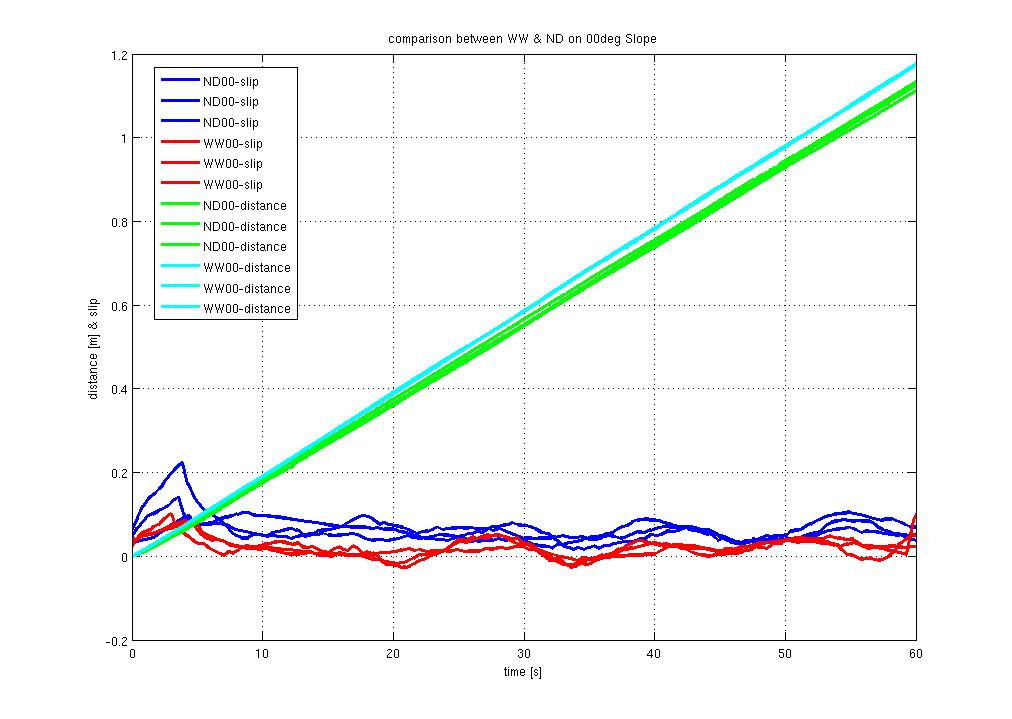
\includegraphics[width=0.9\textwidth]{00d.jpg}
    \caption{Comparison between wheel walking and normal driving on flat terrain}
    \label{fig:00d}
\end{figure}

\subsubsection*{10$^{\circ}$ Tests}
The performance difference in the 10$^\circ$ slope already show the benefit of WW compared to ND. The slip value of former is about 50\% less than in the later case. Still, the slip for both is considered low.

\begin{figure}[h!]
    \centering
    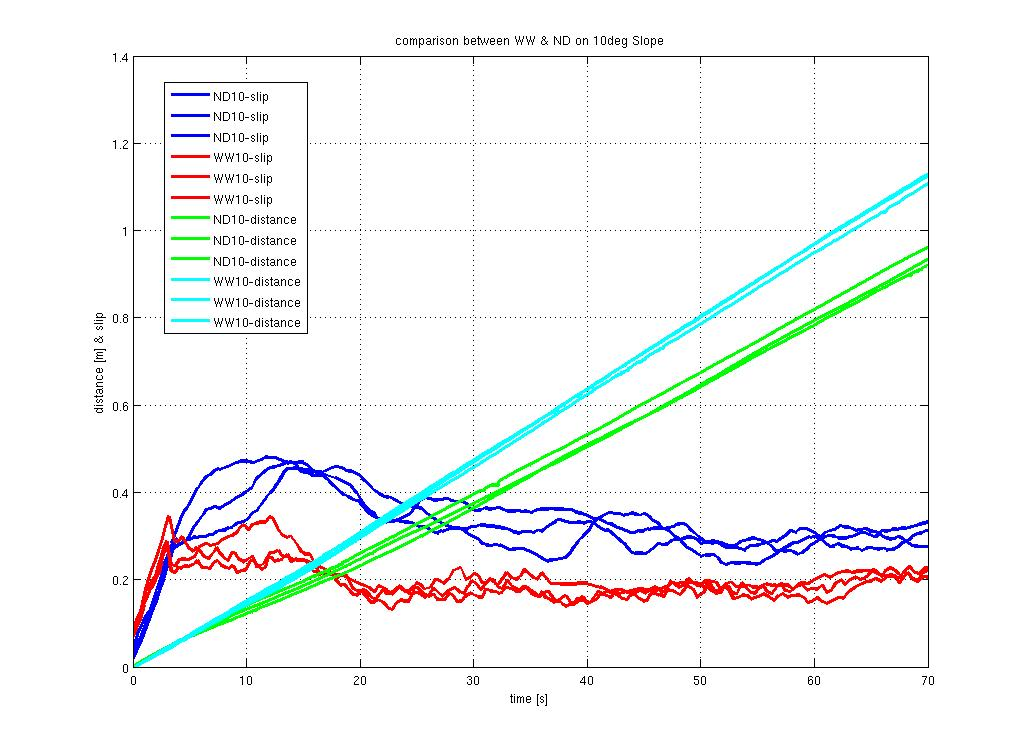
\includegraphics[width=0.9\textwidth]{10d.jpg}	\caption{Comparison between
    wheel walking and normal driving on a 10$^{\circ}$ Slope} \label{fig:10d}
\end{figure}

\subsubsection*{15$^{\circ}$ Tests}
At 15$^\circ$ slope however (see figure \ref{fig:15d}), the difference gets way
more visible in terms of traversed distance.  

\begin{figure}[h!]
    \centering
    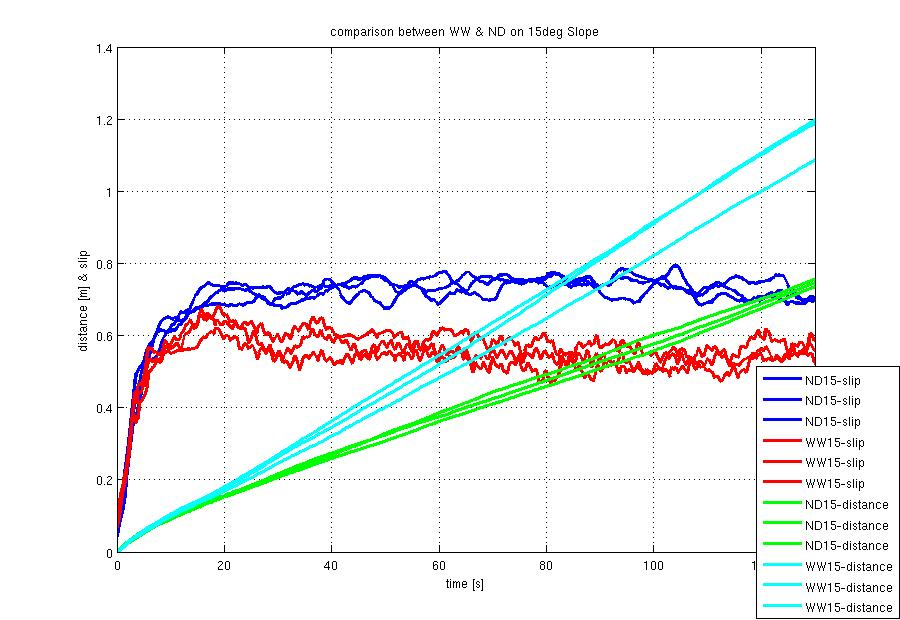
\includegraphics[width=0.9\textwidth]{15d.jpg}	\caption{Comparison between
    wheel walking and normal driving on a 15$^{\circ}$ Slope} \label{fig:15d}
\end{figure}

\subsubsection*{20$^{\circ}$ Tests}
Figure \ref{fig:20d} referring to the 20$^\circ$ slope tests shows the biggest performance difference. The travelled distance is roughly double in case of WW, what means that it has half the average slip. The average slip for WW for the three runs was 82.4\% compared to 89.2\% in the ND (averaged in steady state
from t=75~\unit{s} - t=250~\unit{s}).
The small periodic ripples in the WW runs are generated by the walking motion. While having slip ratios above approximately 10\%, the rover starts waving around a point in between the two rear axes which is not the rover origin. Therefore the tracking shows ripples with a frequency of about 0.7~\unit{Hz}.

\begin{figure}[h!]
    \centering
    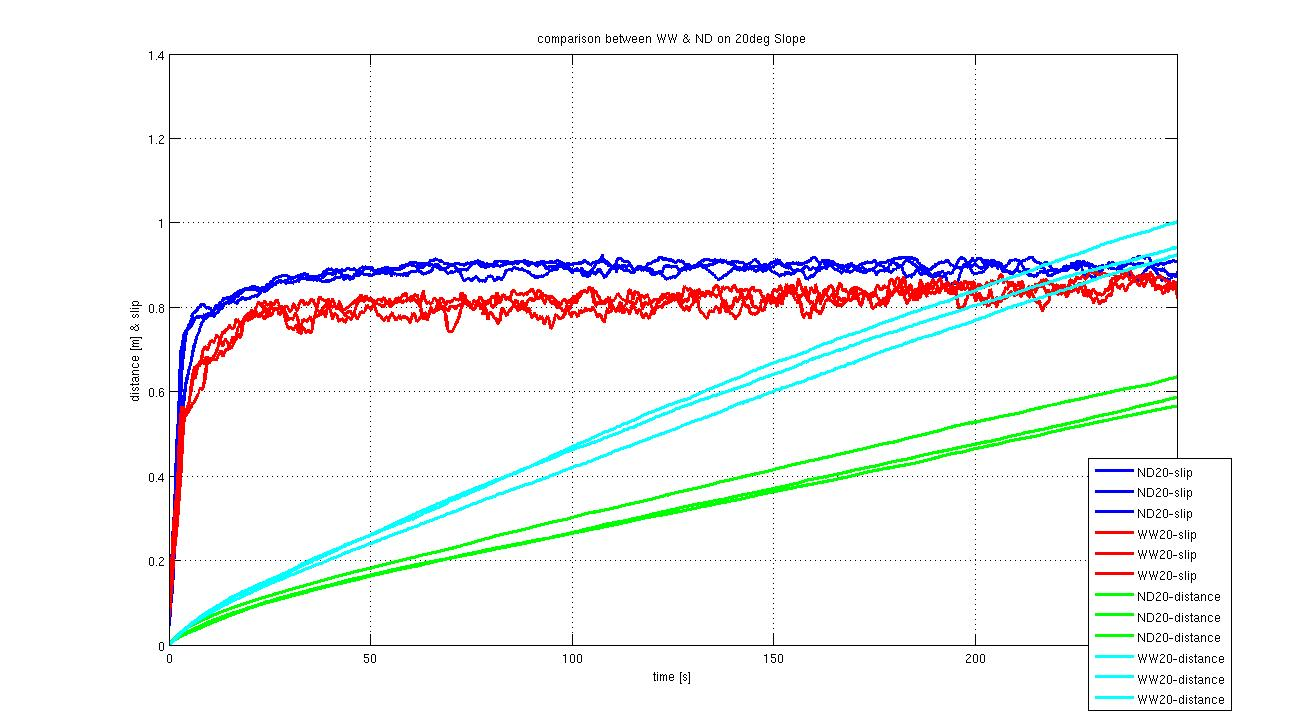
\includegraphics[width=0.9\textwidth]{20d.jpg}	\caption{Comparison between
    wheel walking and normal driving on a 20$^{\circ}$ Slope} \label{fig:20d}
\end{figure}

\subsubsection*{Summary}
Table \ref{tab:SlopeSummaryTable} summarises the results obtained in terms of slip-ratio at each slope angle for ND and WW.

\begin{table}[h]
	\begin{tabular}{lll}
	Slope angle & Avg slip-ratio ND & Avg slip-ratio WW \\
	0$^{\circ}$       & -                 & -                 \\
	10$^{\circ}$      & -                 & -                 \\
	15$^{\circ}$      & -                 & -                 \\
	20$^{\circ}$      & -                 & -                
	\end{tabular}
	\caption{Gradeability tests summary table}
	\label{tab:SlopeSummaryTable}
\end{table}

\subsubsection*{Additional Tests}
A series of tests at 20$^{\circ}$ slope angle were run changing the \textit{step length}\footnotemark[3]
at each run, from 2.5~\unit{cm} to 12.5~\unit{cm} incrementing the step length by 2.5 cm at
each test. The results of these series of tests are inconclusive so far, as no
specific relation can be identified between the step length and the slip ratio.

With the objective of trying to reduce further the slip-ratio, the WW algorithm was modified to include an offset constant rolling speed in all driving motors. This was supposed to increase the traction of "anchoring" wheels during the WW motion. However, this hybrid implementation did not seem to have a positive impact in the slip-ratio.

Other experimental tests include running the system backwards and/or fixing the
walking motors to the position equal to the angular value of the slope. This is
supposed to reduce the load in the back wheels of the rover by shifting the CoM
forward and therefore distribute the weight equally over the three axes and
hence increase in theory the traversability performance. Figure
\ref{fig:ndr20d}) shows the slip ratios obtained for the case of running
backwards with the walking actuators angled in position compared to normal
forward driving. Backward driving here means that the two bogies are in the
back and make an equal load on all four wheels of these bogies due to ExoTeR's
parallel mechanisms. None of these measures shows a clear benefit in the slip-ratio.

\begin{figure}[h!]
    \centering
    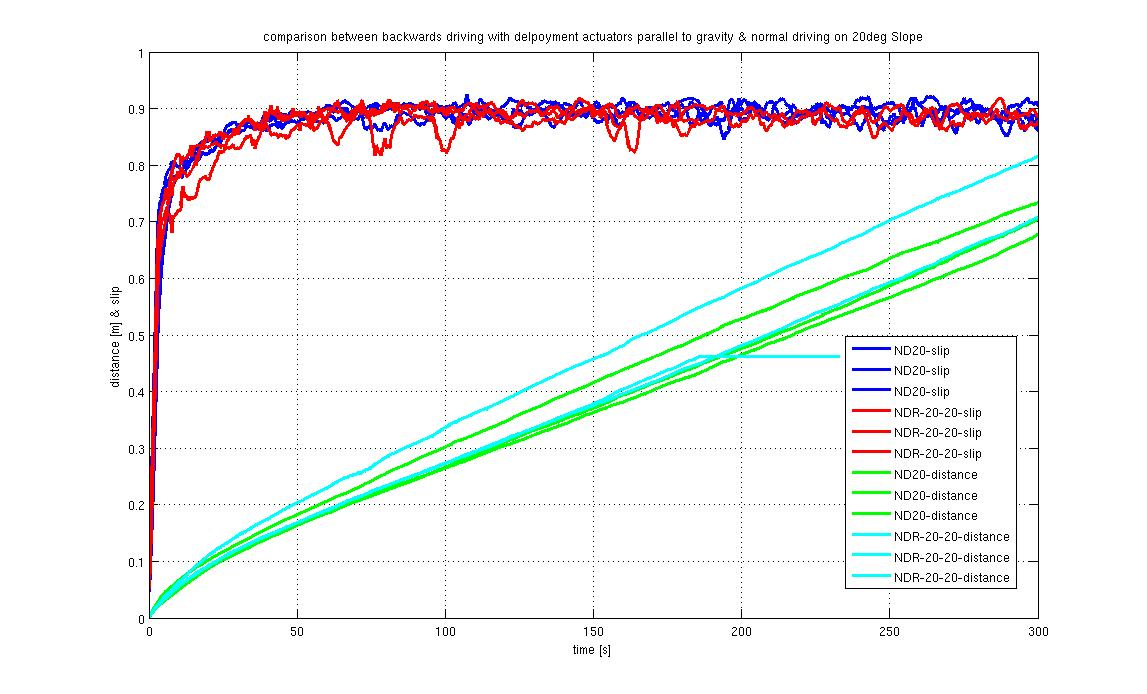
\includegraphics[width=0.9\textwidth]{ndr20d.jpg}	\caption{Comparison between
    normal driving and reverse driving with gravity aligned legs on a 20$^{\circ}$ Slope}
    \label{fig:ndr20d}
\end{figure}

\footnotetext[3]{The step length is here defined as the amount of distance covered by each wheel in a walking sequence.}

%================================================================
%================================================================
\subsection{Lander Egress Tests} 

\subsubsection{Objective}
It is evident that having the "walking" degree of freedom in the control-space of the rover offers more than just performing WW gaits. It allows for configuring the rover posture and shifting the CoM to assist different operations. The objective of this test is to experiment on how the "walking" DoF can assist egress operations from a lander, which is one of the most risky phases of a mission. To simulate these egress conditions, the Planetary Robotics Lab has built an adjustable lander mockup that was loosely based on the preliminary design of the ExoMars lander, appropriately scaled-down to fit the size of the ExoTeR rover. 

\subsubsection{Setup}
The rover egress platform as shown in figures \ref{fig:egress29} \& \ref{fig:egress34} has two egress directions with different ramp lengths and is adjustable in its height. Thereby the egress
angle can be set. It is also adjustable to the track width of the rover. The
ramps are covered with a rubber mat to provide sufficient traction. The
following tests had a step of 8 cm in height at the end of both ramps to simulate
a worst case landing in a rocky environment.  Due to the lack of any designed
flexibility in ExoTeR, the floor is prepared with foam covered by carpet to
absorb part of the impact energy and simulate the behaviour of flexible wheels. It is worth mentioning that the static stability of ExoTeR has been tested and was found to be greater than 40$^\circ$.

At the beginning of the test procedure, the rover is steady on the egress platform and is commanded to drive down with a constant body velocity of 1~\unit{cm/s}. A emergency safety rope is attached to its back and is hand held without tension. 

\begin{figure}[h]
    \centering
    \subfigure{
    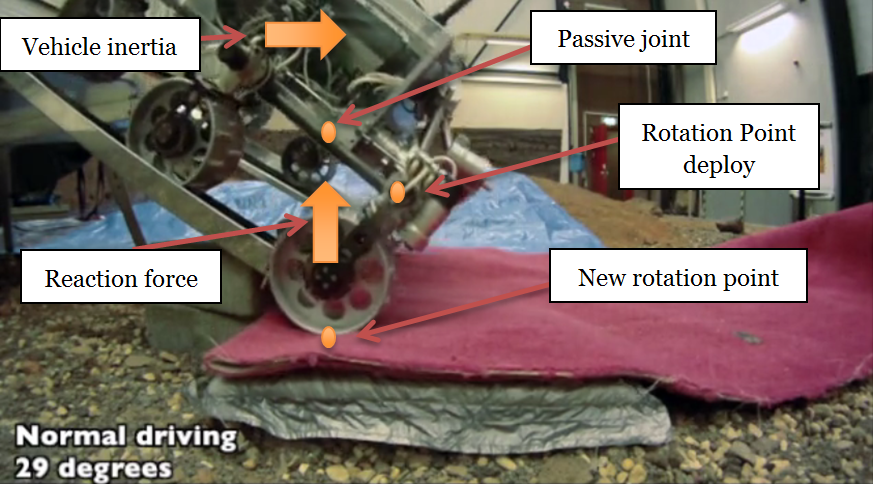
\includegraphics[width=0.9\textwidth]{egress29com.png}	}
    \subfigure{
        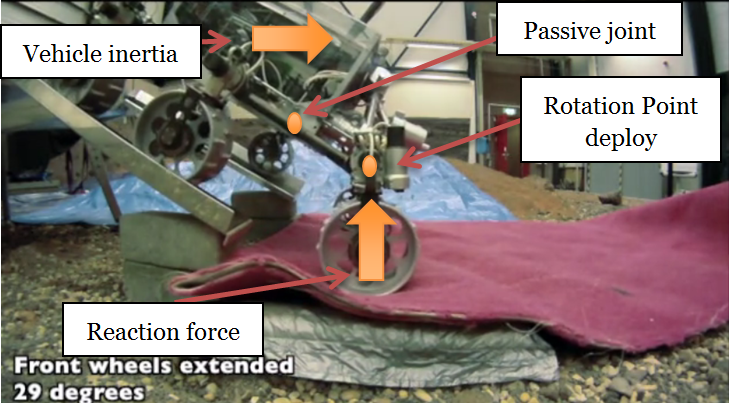
\includegraphics[width=0.9\textwidth]{egress29ext.png}	}
        \caption{Comparison between egressing in normal configuration (top) and
        34$^{\circ}$ forward shifted front wheels (bottom) on a 29$^{\circ}$
        egress ramp with a step at the end} \label{fig:egress29com}
\end{figure}

Figure\ref{fig:egress29com} describes the concept behind this test. The
forward shifting of the front axis should increase the stability of the
whole system due to a bigger horizontal distance between the contact point
on the ground and the CoM. That way the angle at which it tips over is
increased. Second, due to the passive bogie, the maximum angle of egress is
limited to the angle in which the contact point on the ground falls behind
the pivot point of the bogie using their horizontal coordinate. After this
point, the two center wheels would lift off and destabilize the system even
further. In addition, the deployment actuator has to withstand very high
holding torques, both during driving and at the final impact on the ground.
Figure\ref{fig:egress29com}(bottom) has its front axle shifted by
34$^\circ$. The 34 herein is the optimized angle for the 29$^\circ$ ramp
plus the 8 cm drop. 

\subsubsection{Results}
%first the procedure

The tests showed how the dynamic stability of the rover is increased when using
the walking mechanisms to angle the front wheel forward and verified the stated
thesis.  In standard egress manoeuvring, the rover already loses stability
(close to capsize/fall) at the ramp of 26$^\circ$ (see figure
\ref{fig:egress34}(top)) and literally capsizing at the 29$^\circ$ test(see
figure \ref{fig:egress29} - top). Contrary to this, using the walking mechanisms
showed the rover going down keeping constant stability in the 34$^\circ$ ramp
(see figure \ref{fig:egress34}- bottom), which is the maximum possible ramp
for the current setup.

\begin{figure}[h!] \centering
    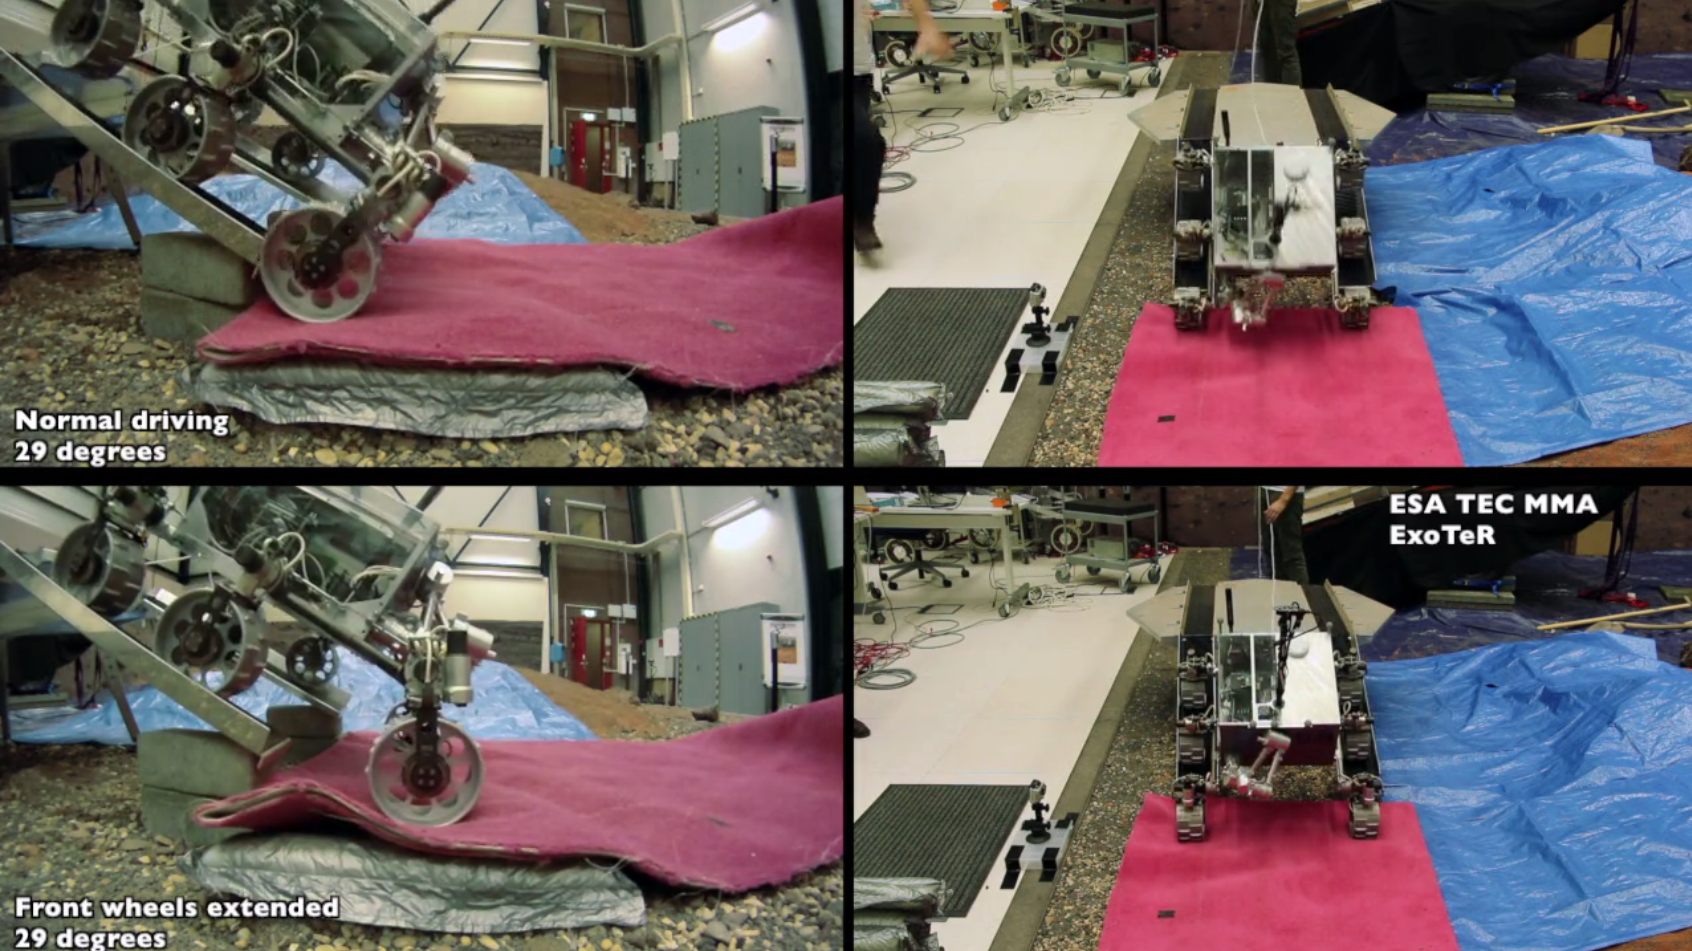
\includegraphics[width=0.9\textwidth]{egress29.png}	\caption{Comparison
    between egressing in normal configuration (top) and 34$^{\circ}$ forward
    shifted front wheels (bottom) on a 29$^{\circ}$ egress} \label{fig:egress29}
\end{figure}

\begin{figure}[h!] \centering
    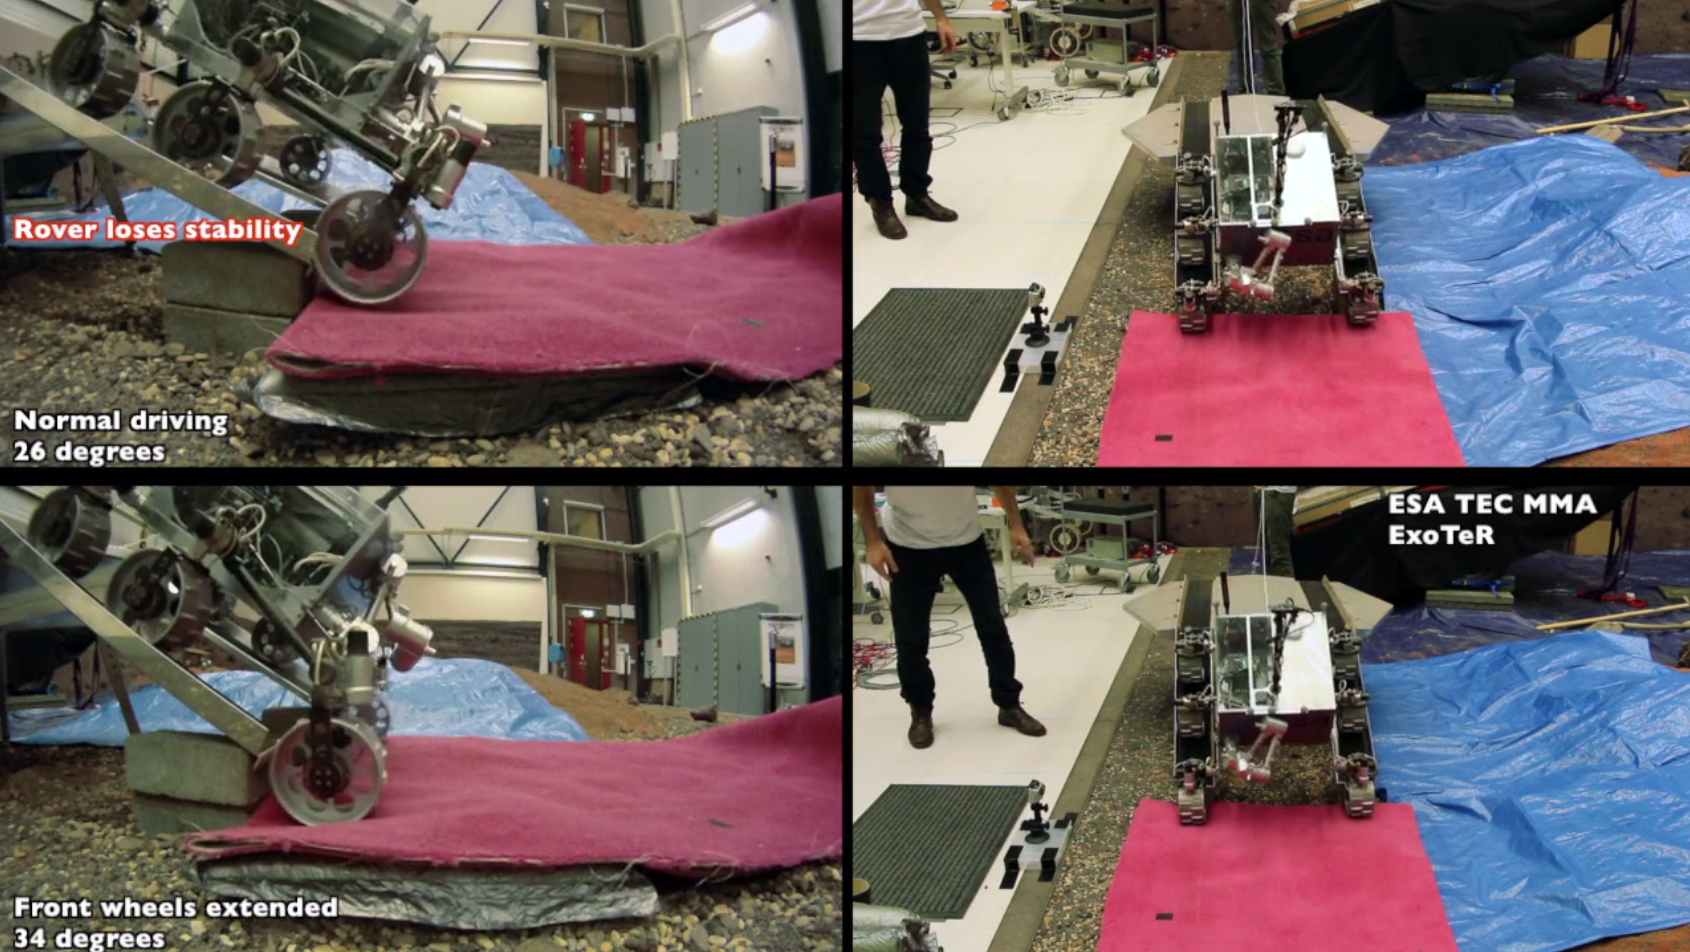
\includegraphics[width=0.9\textwidth]{egress34.png}	\caption{Comparison
    between egressing in normal configuration (top)  on a 26$^{\circ}$ramp
    versus a 39$^{\circ}$ forward shifted front wheels (bottom) on a 34$^{\circ}$
    egress ramp}
    \label{fig:egress34}
\end{figure}

Another side observation is, that the wheel actually drops much less than the
full 8~\unit{cm} of the step height. The traction of the rear four wheels is big enough to
let the front wheel pair roll down smoothly until roughly half of the wheel
diameter, reducing therefore the "free falling" distance.

%================================================================
%================================================================
%\subsection{Results Analysis}

\section{Conclusions}
The wheel-walking locomotion mode outperformed standard rolling in all the
tested scenarios demonstrating better traction in loose soil, increased
gradeability performance and improved dynamic stability limit during egress sequences.
Future rover exploration missions [like ExoMars or Sample Fetching Rover/(specially in the case of systems with high EGP)] could
potentially benefit from the increased locomotion capabilities of wheel-walking
to reduce the chances of getting stuck in loose soil, to enable safe egress
operations or to simply allow a faster or more efficient navigation by reducing
the ground track to straight distance ratio.

\section{Future Work}
Following the results of these first experiments, the Automation \& Robotics Section has decided to
continue this research path and has planned further tests to get more
experimental data and increase the confidence on the performance of wheel-walking.  Future tests will focus on gradeability analysis to better assess the
performance of different wheel-walking gaits in several types of soil.  The
next testing campaign is planned for March 2015 in the Robotics Mechanics
Centre (RMC) of DLR Oberpfaffenhofen.


\vspace{-3 mm}

%%%%%%%%%%%%%%%%%%%%%%%%%%%%%%%%%%%%%%%%%%%%%%%%%%%%%%%%%%%%%%%%%%%%%%%%%%%%%%%%
% \footnotesize
\bibliographystyle{aa}
\bibliography{references}

% \end{small}
\end{document}
